\documentclass[12pt]{article}
\usepackage[utf8]{inputenc}
\usepackage{booktabs}
\usepackage{geometry}
\usepackage{graphicx}
\geometry{a4paper, margin=1in}
\title{Results of the Fisher Combined Test}
\author{Sara Fraija}
\date{\today}
\begin{document}
\maketitle
\section{Resultados}

\begin{table}[h!]
\centering
\resizebox{\textwidth}{!}{%
\begin{tabular}{l c c c c c c}
\toprule
\textbf{GRB} & \textbf{Transit} & \textbf{Significance} & \textbf{Significance Corregida} & \textbf{p-value} & \textbf{Corrected p-value} & \textbf{PDF} \\ \midrule
GRB230812790 & 1 & 0.10 & 0.10 & 5.398e-01 & 4.602e-01 & 6.030e-01 \\
GRB160612842 & 1 & 0.00 & -0.00 & 5.000e-01 & 5.000e-01 & 6.011e-01 \\
GRB160821937 & 1 & 1.95 & 1.95 & 9.744e-01 & 2.559e-02 & 9.404e-01 \\
GRB150120123 & 1 & 1.90 & 1.90 & 9.713e-01 & 2.872e-02 & 9.344e-01 \\
GRB180418281 & 1 & 1.11 & 1.11 & 8.665e-01 & 1.335e-01 & 7.845e-01 \\
GRB181125371 & 1 & 0.00 & -0.00 & 5.000e-01 & 5.000e-01 & 6.011e-01 \\
GRB230512269 & 1 & 0.81 & 0.81 & 7.910e-01 & 2.090e-01 & 7.126e-01 \\
GRB170708046 & 1 & 0.97 & 0.26 & 8.340e-01 & 3.961e-01 & 7.508e-01 \\
GRB210827416 & 1 & 0.24 & 0.24 & 5.948e-01 & 4.052e-01 & 6.124e-01 \\
GRB180805543 & 1 & 0.11 & 0.11 & 5.438e-01 & 4.562e-01 & 6.035e-01 \\
GRB220412713 & 1 & 1.15 & 1.15 & 8.749e-01 & 1.251e-01 & 7.941e-01 \\
GRB170826369 & 1 & 1.58 & 0.31 & 9.429e-01 & 3.802e-01 & 8.855e-01 \\
GRB180204109 & 1 & 1.74 & 1.74 & 9.591e-01 & 4.093e-02 & 9.122e-01 \\
GRB201214672 & 1 & 2.85 & 2.85 & 9.978e-01 & 2.186e-03 & 9.931e-01 \\
GRB160624477 & 1 & 0.88 & 0.88 & 8.106e-01 & 1.894e-01 & 7.291e-01 \\
GRB151229285 & 1 & 1.10 & 1.10 & 8.643e-01 & 1.357e-01 & 7.821e-01 \\
GRB220617772 & 1 & 0.24 & 0.24 & 5.948e-01 & 4.052e-01 & 6.124e-01 \\
GRB150110923 & 1 & 1.67 & 1.67 & 9.525e-01 & 4.746e-02 & 9.011e-01 \\
GRB180715755 & 1 & 0.95 & 0.95 & 8.289e-01 & 1.711e-01 & 7.459e-01 \\
GRB190515190 & 1 & 0.00 & -2.92 & 5.000e-01 & 9.982e-01 & 6.011e-01 \\
GRB170318644 & 1 & 0.00 & -0.00 & 5.000e-01 & 5.000e-01 & 6.011e-01 \\
GRB230228244 & 1 & 0.00 & -0.00 & 5.000e-01 & 5.000e-01 & 6.011e-01 \\
GRB170403583 & 1 & 0.00 & -2.00 & 5.000e-01 & 9.770e-01 & 6.011e-01 \\
GRB211024065 & 1 & 0.00 & -0.00 & 5.000e-01 & 5.000e-01 & 6.011e-01 \\
GRB221120895 & 1 & 0.75 & 0.75 & 7.734e-01 & 2.266e-01 & 6.989e-01 \\
GRB220511571 & 1 & 1.70 & 1.70 & 9.554e-01 & 4.457e-02 & 9.060e-01 \\
GRB220418720 & 1 & 0.83 & 0.83 & 7.967e-01 & 2.033e-01 & 7.173e-01 \\
GRB190427190 & 1 & 2.59 & 2.59 & 9.952e-01 & 4.799e-03 & 9.861e-01 \\
GRB201008443 & 1 & 2.22 & 2.22 & 9.868e-01 & 1.321e-02 & 9.661e-01 \\
GRB170803729 & 1 & 0.28 & 0.28 & 6.103e-01 & 3.897e-01 & 6.164e-01 \\
GRB150101641 & 1 & 1.46 & 1.46 & 9.279e-01 & 7.215e-02 & 8.626e-01 \\
GRB210323918 & 1 & 0.00 & -0.00 & 5.000e-01 & 5.000e-01 & 6.011e-01 \\
GRB170817529 & 1 & 2.54 & 2.54 & 9.945e-01 & 5.543e-03 & 9.842e-01 \\
GRB170816599 & 1 & 1.69 & 1.17 & 9.545e-01 & 1.214e-01 & 9.043e-01 \\
GRB180718082 & 1 & 1.61 & 1.61 & 9.463e-01 & 5.370e-02 & 8.908e-01 \\
GRB230228244 & 2 & 1.26 & 1.26 & 8.962e-01 & 1.038e-01 & 8.196e-01 \\
GRB220412713 & 2 & 1.29 & 1.29 & 9.015e-01 & 9.853e-02 & 8.264e-01 \\
GRB220617772 & 2 & 1.91 & 1.91 & 9.719e-01 & 2.807e-02 & 9.356e-01 \\
GRB190515190 & 2 & 2.07 & 0.98 & 9.808e-01 & 1.626e-01 & 9.532e-01 \\
GRB221120895 & 2 & 0.77 & 0.77 & 7.794e-01 & 2.206e-01 & 7.034e-01 \\
GRB170826369 & 2 & 3.03 & 2.33 & 9.988e-01 & 9.912e-03 & 9.960e-01 \\
GRB150101641 & 2 & 0.44 & 0.44 & 6.700e-01 & 3.300e-01 & 6.379e-01 \\
GRB170318644 & 2 & 1.25 & 1.25 & 8.944e-01 & 1.056e-01 & 8.174e-01 \\
GRB170816599 & 2 & 1.92 & 1.44 & 9.726e-01 & 7.435e-02 & 9.368e-01 \\
GRB220511571 & 2 & 2.47 & 2.47 & 9.932e-01 & 6.756e-03 & 9.811e-01 \\
GRB181125371 & 2 & 1.31 & 1.31 & 9.049e-01 & 9.510e-02 & 8.309e-01 \\
GRB180805543 & 2 & 1.77 & 1.77 & 9.616e-01 & 3.836e-02 & 9.167e-01 \\
GRB201214672 & 2 & 2.11 & 2.11 & 9.826e-01 & 1.743e-02 & 9.569e-01 \\
GRB170206453 & 2 & 0.16 & -2.33 & 5.636e-01 & 9.900e-01 & 6.061e-01 \\
GRB150819440 & 2 & 1.41 & 0.82 & 9.207e-01 & 2.050e-01 & 8.524e-01 \\
GRB230812790 & 2 & 1.24 & 1.24 & 8.925e-01 & 1.075e-01 & 8.151e-01 \\
GRB171007498 & 2 & 0.00 & -0.00 & 5.000e-01 & 5.000e-01 & 6.011e-01 \\
GRB151229285 & 2 & 1.01 & 1.01 & 8.438e-01 & 1.562e-01 & 7.604e-01 \\
GRB201008443 & 2 & 1.96 & 1.96 & 9.750e-01 & 2.500e-02 & 9.416e-01 \\
GRB180418281 & 2 & 2.19 & 2.19 & 9.857e-01 & 1.426e-02 & 9.637e-01 \\
GRB150110923 & 2 & 2.10 & 2.10 & 9.821e-01 & 1.786e-02 & 9.560e-01 \\
GRB160714097 & 2 & 0.00 & -0.00 & 5.000e-01 & 5.000e-01 & 6.011e-01 \\
GRB210827416 & 2 & 0.00 & -0.00 & 5.000e-01 & 5.000e-01 & 6.011e-01 \\
GRB210323918 & 2 & 0.08 & 0.08 & 5.319e-01 & 4.681e-01 & 6.023e-01 \\
GRB220418720 & 2 & 2.48 & 2.48 & 9.934e-01 & 6.569e-03 & 9.816e-01 \\
GRB230512269 & 2 & 0.00 & -0.00 & 5.000e-01 & 5.000e-01 & 6.011e-01 \\
GRB200605762 & 2 & 1.01 & 0.02 & 8.438e-01 & 4.932e-01 & 7.604e-01 \\
GRB180718082 & 2 & 2.76 & 2.76 & 9.971e-01 & 2.890e-03 & 9.912e-01 \\
GRB210618072 & 2 & 1.20 & 1.20 & 8.849e-01 & 1.151e-01 & 8.058e-01 \\
GRB170803729 & 2 & 1.22 & 1.22 & 8.888e-01 & 1.112e-01 & 8.105e-01 \\
GRB190427190 & 2 & 0.00 & -0.00 & 5.000e-01 & 5.000e-01 & 6.011e-01 \\
GRB160612842 & 2 & 0.01 & 0.01 & 5.040e-01 & 4.960e-01 & 6.011e-01 \\
GRB170817529 & 2 & 1.68 & 1.68 & 9.535e-01 & 4.648e-02 & 9.027e-01 \\
GRB160624477 & 2 & 1.89 & 1.89 & 9.706e-01 & 2.938e-02 & 9.331e-01 \\
GRB180204109 & 2 & 0.95 & 0.95 & 8.289e-01 & 1.711e-01 & 7.459e-01 \\
GRB170403583 & 2 & 1.69 & 0.76 & 9.545e-01 & 2.240e-01 & 9.043e-01 \\
GRB200623138 & 2 & 0.00 & -0.00 & 5.000e-01 & 5.000e-01 & 6.011e-01 \\
GRB180715755 & 2 & 0.49 & 0.49 & 6.879e-01 & 3.121e-01 & 6.462e-01 \\
GRB180402406 & 2 & 2.02 & 2.02 & 9.783e-01 & 2.169e-02 & 9.481e-01 \\
GRB170708046 & 2 & 0.86 & 0.12 & 8.051e-01 & 4.524e-01 & 7.244e-01 \\
\bottomrule
\end{tabular}%
}
\caption{Lista de GRBs with sus Transits, Significances, Significances Corregidas, p-values, p-values Corregidos y valores PDF.}
\end{table}

\begin{figure}[h!]
\centering
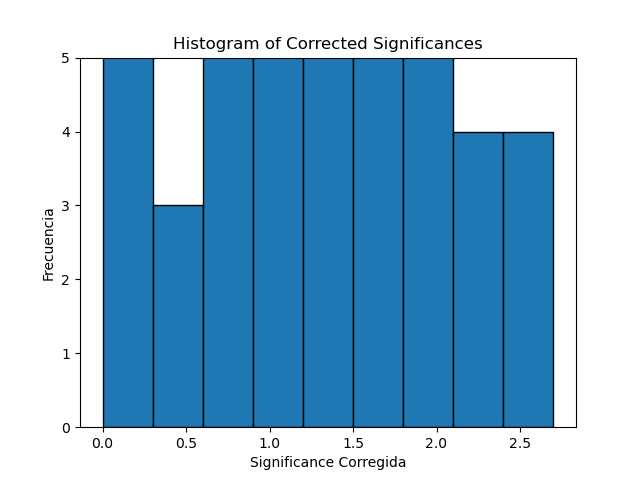
\includegraphics[width=0.6\textwidth]{corrected_significance_hist.png}
\caption{Histogram of Corrected Significances.}
\end{figure}

\section*{Conclusion}
The Fisher combined test integrates individual p-values to evaluate a global hypothesis.
The resulting test statistic was $X^2 = 322.664$ with 150 degrees of freedom.
For a significance level of 0.05, the critical value is 179.581.
Since $X^2$ is greater than the critical value, we rechazamos the null hypothesis of independence.
Normal approximation: p-value = 1.529e-14, significance ≈ 7.60 sigma.

\end{document}